\documentclass[a4paper]{article}
\usepackage[utf8]{inputenc}

\usepackage{a4wide}
\usepackage{url}

\usepackage{alltt}
% Hmmm... Do not work with UTF-8:
% \usepackage{verbatim}

\usepackage{listings}%[hyper,procnames]
\lstset{extendedchars=true, language=C++, basicstyle=\scriptsize\ttfamily, numbers=left,
  numberstyle=\tiny, stepnumber=5, numberfirstline=true,
  tabsize=8, tab=\rightarrowfill, keywordstyle=\bf,
  stringstyle=\rmfamily, commentstyle=\rmfamily\itshape}

\usepackage{abbrev_reactive}
\let\OldRightarrow=\Rightarrow
\RequirePackage{marvosym}
\let\MarvosymRightarrow=\Rightarrow
\let\Rightarrow=\OldRightarrow
\RequirePackage{wasysym}
\let\Lightning\UnTrucIndefini% Car conflit entre ifsym et marvosym
\let\Sun\UnTrucIndefini%
\RequirePackage[weather]{ifsym}


\newcommand{\LINK}[1]{\url{#1}\xspace}
\newcommand{\PfaOrganizationPDF}{\LINK{http://download.par4all.org/doc/developer_guide/par4all_organization.pdf}}
\newcommand{\PfaAllOrganizationHTDOC}{\LINK{http://download.par4all.org/doc/developer_guide/par4all_organization.htdoc}}

\sloppy

% Number everything in the TOC:
\setcounter{secnumdepth}{10}
\setcounter{tocdepth}{10}

\begin{document}

\title{Par4All developer guide\\
  ---\\
  HPC Project}

\author{Amaury \textsc{Darsch} \and Serge \textsc{Guelton} \and Ronan
  \textsc{Keryell} \and Grégoire \textsc{Péan} \and Claire \textsc{Seguin}
  \and Mickaël \textsc{Thievent} \and Pierre \textsc{Villalon}}

\maketitle

% The version is here and not in the title to avoid triggering a bug in
% tex4ht:
\noindent\textbf{This manual is for \Apfa version ../../VERSION}
\bigskip

This document can be found in PDF format on \PfaOrganizationPDF and in HTML
on \PfaAllOrganizationHTDOC.

% To automatically build reports from this content:
%%ContentBegin

\section{Introduction}
\label{sec:introduction}

\Apfa is a platform that merges various open source developments to ease
the migration of sequential software to multicore and other parallel
processors.

\Apfa is mainly developed by \Ahpcp, MINES ParisTech/\Acri, Institut
Télécom/Télécom Bretagne and others.

This document describes the internal organization of \Apfa and how its
construction relies on \Agit repositories, \Asvn repositories and other
projects.

This document describes also the internal workings of \Apfa.
This information may be useful not only for \Apfa core developers but
also for advanced users desiring more functionality from \Apfa.

Since \Apfa relies on other tool projects, the documentation of these other
projects should also be consulted independently and is not included here.

The first section contains the release notes for \Apfa, including
installations instructions. For detailed information on \Apfa
infrastructure, including instructions for compilation, see
sections~\ref{sec:compilation} and above.

\tableofcontents{}

\bigskip{}

\section{Advanced installation using git}
\label{sec:advanced_installation}

For a more simple installation please refer to \url{{http://download.par4all.org/doc/installation_guide}.

The classical \Aautotools environment variables can be used to influence
the compilation, however, some are directly set up from the \verb|p4a_setup.py|
script. Therefore, to set the \texttt{CFLAGS} and \texttt{CPPFLAGS}
to compile \Apfa in debug mode, value changes should be passed through
a \verb|p4a_setup.py| option. For example,
\begin{verbatim}
--configure-options="CFLAGS='-ggdb -g3 -Wall -std=c99'"
\end{verbatim}
sets debugging options that allow \texttt{gdb} to access macro
definitions that are heavily used in \Apips. Indeed this case is so common
when debugging \Apfa that the \verb|--debug| or \verb|-g| options are just
doing this for simplicity.

The installation process can be modified by passing options to
\verb|p4a_setup.py|. For example, to skip the (re)compilation of the
package \texttt{polylib},
\verb/--skip-polylib/) is used. The complete set of options is described in
\S~\ref{sec:p4a_s-comp-script}.

The \texttt{make} command has options for speeding up the compilation. For
example, to run on 8 processes, the \verb/--jobs=8/ option is added.

To compile \Apfa directly from source packages that are not
inside the \Apfa directory hierarchy, see \S~\ref{sec:direct-organ}. In
this case, \texttt{-{}-\emph{PACKAGE}-src=...} specifies the
location of the sources of \texttt{\emph{package}}, (e.g.,
\verb|-pips-src=...| or \verb|--polylib-src=...|). If all these options are
set (e.g., if the source locations point to working copies of the
\Apips{} \Asvn), then the \texttt{p4a-own} branch can be used for
compilation. For the \Apips
packages, there must be links to \texttt{nlpmake/makes} to enable compilation.
See \S~\ref{sec:comp-from-sourc} for more information on alternate
source locations.

The options passed to \texttt{configure} for a package can be changed by
using the \texttt{-{}-\emph{PACKAGE}-conf-options=...}

For example, to compile \Apips with Fortran 95 support, use:
\begin{verbatim}
p4a_setup.py --only=pips --pips-conf-options="--enable-tpips --enable-pyps \
  --enable-hpfc --enable-fortran95" --reconf --no-final
\end{verbatim}

To recompile and intall \Apips after subsequent modifications, use:
\begin{verbatim}
p4a_setup.py --only=pips --no-final
\end{verbatim}

Beware that if \verb|--pips-src| is used to designate a \Apips
directory that has been previously build in a classical way (such as
the classical \Asvn build), the compilation will fail because of
incorrect dependencies between the files contained therein (which are not
related to \Apfa \texttt{build} directory location). Prior to running
the script, run the following in the \Apips source directory.
\begin{verbatim}
make clean
\end{verbatim}

To recompile a part of \Apfa (for example to debug
one of the components) without using \verb|p4a_setup.py|, change to
the directory \verb|$P4A_ROOT/build| in the relevant component. For
example, change to \verb|$P4A_ROOT/build/newgen| and type:
\begin{verbatim}
make
\end{verbatim}
and upon completion, type:
\begin{verbatim}
make install
\end{verbatim}
to complete the build process. The direct \texttt{install}
approach can be used to avoid testing the compilation
\emph{a priori}. However, the 2-step
approach is most useful if, for example, there is a debug session or a
validation on the installed version and at the same time, a parallel
development and verification effort. One can work in the latter
without invalidating the running version.

\subsection{The \protect\texttt{p4a\_setup.py} compilation and installation
script}
\label{sec:p4a_s-comp-script}

The compilation and installation of \Apfa is controlled by the
\verb|p4a_setup.py| script, with the usage and options described in
this section.

\input{p4a_setup-help}

\section{Committing using git}

In general, to commit changes to the \Agit repository, the
\texttt{p4a-own} branch should be used and not any of the \Apfa
sub-packages. If a branch must be used, see section~\ref{sec:packages}
to ensure consistency with the \Apfa compilation process. It is highly
advisable to compile work before
committing it on the central repositories and to make sure that all
files are committed so that the code compiles in all user
environments. In addition to providing
consistency, this has the added advantage of
allowing one to test one's code before releasing it for general
consumption! \smiley

A nice feature of \Agit over \Asvn is that since the commit is separated from
the publication, a commtted state can be tested independently from the
rest of the team before pushing to the global server.

For example, one can create a light\footnote{Because the objects are
  shared with symbolic links and not copied, since we did not use the
  \texttt{file://} syntax.} clone with
\begin{verbatim}
git clone --branch p4a par4all par4all-compile
\end{verbatim}
and after testing and committing modifications inside the
\texttt{par4all} working copy, one does the same into the
\texttt{par4all-compile} working copy after a \texttt{git pull}.
If some files are lacking from the commit, \Agit will be detect the discrepancy.

Afterwards, a \texttt{git push} into the central \Apfa
repository will have fewer associated risks.


\section{Collaborative repositories}
\label{sec:coll-repos}


\subsection{Public repositories}
\label{sec:public-repositories}

There are several \Agit repositories used by the project.

To have access without authentication and only for reading/cloning, use
the \texttt{git:} prefix instead of \texttt{ssh:}, e.g.,
\url{git://git.hpc-project.com/git/par4all.git}.

The main repository for the project is located at
\url{ssh://git.hpc-project.com/git/par4all.git}

This repository can be viewed with a \Awww browser at
\url{https://git.hpc-project.com/cgit/par4all}

To get directly involved into the project with full commit capability
directly into the repositories, ask \Ahpcp.

There are also ancillary \Agit repositories that provide a \Agit interface to
the trunk of the \Asvn repositories for the \Apips components from
\Acri:
\begin{itemize}
\item \url{ssh://git.hpc-project.com/git/svn-linear.git}
\item \url{ssh://git.hpc-project.com/git/svn-newgen.git}
\item \url{ssh://git.hpc-project.com/git/svn-nlpmake.git}
\item \url{ssh://git.hpc-project.com/git/svn-pips.git}
\item \url{ssh://git.hpc-project.com/git/svn-validation.git}
\end{itemize}
These ancillary gateways only include the \texttt{trunk} history since the
\Acri branches are not public.

In the case of \texttt{nlpmake}, another \Agit{} \Asvn gateway at the top
level has been used for the integration with \texttt{trunk},
\texttt{branch} and \texttt{tag}. This is due to the fact that
\texttt{nlpmake} started without the standard
layout, which was added later at approximately revision 750. Because
of this prior history, this gateway is not published in a public git.

\subsection{Private repositories}
\label{sec:private-repositories}

There is a private directory shared between core developers and used mainly
for validation of the project on non public codes, benchmarks, demos,
and for developing private reports, phases, scripts and so on:
\url{ssh://git.hpc-project.com/git/par4all-private.git}

For \Ahpcp-confidential information,
\url{ssh://git.hpc-project.com/git/par4all-private-hpc.git} is used.

Other repositories can be created and used on demand according to the
needs of evolving private collaborations.

\subsection{Packages}
\label{sec:packages}

\Apfa integrates different tools from different projects. Currently, \Apfa
is composed of \Apips, \Apipsgfc, \Apolylib, with some extensions. Each
project is included in \Apfa as a package and is placed in a directory
inside the \texttt{package} top-level directory.
These directories exist as \Agit subtrees to ease revision control and
integration, even when not connected to the \Asvn server.

Since \Apfa is an integration project, to modify or develop in
a particular package, please work in the upstream package and not in
\Apfa\footnote{In fact, this method is used for \Apfa development at Rensselaer
  Polytechnic Institute; global developments in \Apips are created
  directly and easily into \texttt{package/PIPS}. However,
  the re-integration becomes more difficult since it requires extracting the
  patch history in \texttt{package/PIPS} and merging it into the \Apips
  upstream \Asvn repository.}. Working in this manner facilitates
compilation of \Apfa with package sources outside of \Apfa (see
\S~\ref{sec:p4a_s-comp-script}), which can be committed into their own upstream
version control systems.


\subsection{Directory organization}
\label{sec:direct-organ}
The \Apfa distribution contains the following directories:

\begin{description}
\item[\texttt{build}] is created when compiling the various
  \Apfa packages from the \Aautotools;
\item[\texttt{doc}] contains the sources of the \Apfa documentation,
  including those for the user and the programmer as well as those
  about the infrastructure:
  \begin{description}
  \item[\texttt{organization}] stores indeed the sources of this document;
  \item[\texttt{p4a\_coding\_rules}] contains some coding rules
    applications should respect to be dealt seamlessly by \Apfa;
  \item[\texttt{simple\_tools/p4a\_article}] describes the \Apfa
    capabilities for the end user and is the user manual;
  \item[\texttt{p4a\_slides}] is a very simplified version of the previous
    manual as slides;
  \end{description}
\item[\texttt{examples}] contains some examples and benchmarks to exercise
  \Apfa. These examples also encompass \Apfa demos;
\item[\texttt{packages}] contains the different components of \Apfa:
  \begin{description}
  \item[\texttt{PIPS}] contains the components of \Apips framework
    itself, including:
    \begin{description}
    \item[\texttt{linear}:] the main linear library of \Apips;
    \item[\texttt{newgen}:] the object management infrastructure used by
      \Apips;
    \item[\texttt{nlpmake}:] the makefile common infrastructure used by
      all the \Apips components
    \item[\texttt{pips}:] the \Apips core;
    \item[\texttt{validation}:] the validation of \Apips;
    \end{description}
  \item[\texttt{pips-gfc}] contains a \Agcc 4.4 source patch to be
    compiled and linked with \Apips that adds a Fortran 95+ parser to \Apips;
  \item[\texttt{polylib}] contains the \Apolylib linear library source;
  \end{description}
\item[\texttt{src}] contains sources of tools used for the internal
  organization of \Apfa itself, such as repository and product management,
  product publication, or run-time management (e.g., \verb|p4a_accel|);
\item[\texttt{\emph{PREFIX-DIR}}] contains the usable \Apfa is installed
  after compilation:
  \begin{description}
  \item[\texttt{bin}] contains the executable programs from \Apfa;
  \item[\texttt{doc}] contains the generated documentation for the \Apfa
    infrastructure;
  \item[\texttt{etc}] contains some generated configuration files;
  \item[\texttt{examples}] contains with some examples to exercise \Apfa;
  \item[\texttt{include}] contains the include files used for the
    compilation of \Apfa;
  \item[\texttt{lib}] contains the libraries used to run \Apfa;
  \item[\texttt{makes}] contains \texttt{make}-file tools for the
    \Apips validation;
  \item[\texttt{RELEASE-NOTES.txt}] is the release notes of this \Apfa
    instance;
  \item[\texttt{share}] contains shared files for run-time and
    configuration files
  \item[\texttt{VERSION}] is the current version of this \Apfa
    instance.
  \end{description}
\end{description}


\section{Repositories and work-flow}
\label{sec:repos-workfl}

For history tracking and collaborative development, \Apfa relies on a main
\Agit repository that is accessed by \Apfa developers, users, integrators,
and the production and quality assurance team.

The script \verb|p4a_git| is used to automate the management of the
workflow.

Since \Apfa extends some tools such as \Apips, their are some
ancillary repositories to ease the impedance matching between \Apfa and
those other projects.

Since \Apolylib is already a \Agit repository, it is simply fetched as a
remote \Agit into the \Apfa at the right place.

The process is more complex with \Apips, which is a project split in 5
independent \Asvn repositories requiring more effort for coherent presentation.
Toward this end, \Asvn-\Agit gateways are used to offer freedom of
development and independence from other review hierarchies. Using
these dateways, light
branches are stored into a common \Agit view of the \Apips{} \Asvn
repositories; these light branches can be pushed back into the \Apips{} \Asvn.

\subsection{The p4a\_git script to deal with workflow}
\label{sec:p4a_git-script-deal}

The \verb|p4a_git| script is used to manage the workflow of \Apfa
involving all the related \Agit and \Asvn repositories.

For easy rollback to a robust state, a branch can be created with
\texttt{git checkout -b} and tested independently prior to merging
with the public repository. If the independent branch fails, then it
can be deleted without impacting other work.
See the \texttt{git reset} documentation for more details.

Some use cases of \verb|p4a_git| require that the \verb|P4A_TOP|
environment variable be set to the top directory of the \Apfa
infrastructure wherein reside the various \Agit working copies involved in the
project.

The following section presents some examples, after which the full
list of options is described in detail.

\subsubsection{\protect\texttt{p4a\_git} and \protect\texttt{git} typical use cases}
\label{sec:p4a_git-typical-use}

The \Apfa \texttt{p4a} reference branches are used to contstruct \Apfa
and potentially contain integration work performed by \Apfa team
members beyond the current release. To retrieve an up-to-date version
of a reference branch, use:
\begin{verbatim}
p4a_git --branch-action "git checkout p4a\$suffix; git pull origin p4a\$suffix"
\end{verbatim}

Work performed on \Apfa itself without integrating new versions of upstream
packages is first integrated into the \texttt{p4a-own} branch using:
\texttt{git} stuff:
\begin{verbatim}
git checkout p4a
git merge p4a-own
\end{verbatim}
When the results are validated and reread (for example verify with
\texttt{gitk} that something has not been committed by error on
\texttt{p4a} branch), work is published to the main \texttt{p4a} branch
using:
\begin{verbatim}
git push origin p4a-own
git push origin p4a
\end{verbatim}

A typical example to build a \Apfa with the latest \Apips version into the
reference \verb|p4a| branch infrastructure (after having merged
reference branches as explained previously) is as follows:
\begin{verbatim}
p4a_git --build-new-p4a
\end{verbatim}

Indeed, the effect is to chain the following actions that can be manually
used to tweak the aggregation process (for example to skip a wrong or
out-of-phase commit in \Apips):
\begin{itemize}
\item fetch the most recent developments of upstream packets (\Apips,
  \Apolylib...) into the \texttt{git svn} repositories in the
  \texttt{CRI-git-svn} folder:
\begin{verbatim}
p4a_git --update-git-svn
\end{verbatim}
\item merge the new versions of the upstream packages into the \Apfa
  reference branches, such as \texttt{CRI-pips}:
\begin{verbatim}
p4a_git --fetch-remote-git
\end{verbatim}
\item pull all the component branches (such as \texttt{CRI-pips}) into the
  \Apfa integration branch hierarchy (such as \texttt{p4a-pips}):
\begin{verbatim}
p4a_git --pull-remote-git
\end{verbatim}
  This is where you can play around upstream flows. For example you can
  afterwards send the \texttt{p4a-pips} back a few commits, cherry-pick
  from \texttt{CRI-pips} some useful contributions among broken commits.

  Note that the 2 previous instructions work into \verb|$P4A_ROOT|, %$
  so make sure it does not point to a default installation directory such
  as \texttt{/usr/local/par4all}. You can update \verb|$P4A_ROOT| %$
  or use the \verb|--root .| option if you worked in the \texttt{par4all}
  working copy;
\item fuse all the component branches into the \Apfa integration
  branch hierarchy:
\begin{verbatim}
p4a_git --aggregate-branches
\end{verbatim}
\end{itemize}

At the end of this sequence of steps, the most recent developments in all
parts of \Apfa is contained in the \verb|p4a| branch infrastructure.
After testing and validation, this branch can be published\footnote{But
  before this, think to verify it is correct with a tool like
  \texttt{gitk} because it may be cumbersome for the community to remove
  some wrongly pushed commits...}  as the latest official version with:
\begin{verbatim}
p4a_git --branch-action git push origin \$branch
\end{verbatim}
If someone else updates a branch in the meantime, the new branches
must be merged back into the local versions by re-executing the sequence
of steps at the beginning of this section.

\subsubsection{More advanced use cases for \protect\texttt{p4a\_git}}
\label{sec:more-advanced-use}

The previous section provides enough guidance for simple integration
and maintenance of \Apfa. In this section, more advanced use cases are
presented.

The developer can create from \texttt{p4a} a branch infrastructure
\verb|p4a-very-personal|, with \verb|p4a-very-personal-pips| for
\Apips, \verb|p4a-very-personal-polylib| for \Apolylib, etc.,
with each attached to the main \verb|p4a|-prefixed branch
infrastructure. To do this, use;
\begin{verbatim}
p4a_git --aggregate-branches p4a-very-personal
\end{verbatim}

To start from \texttt{p4a-0.2-alpha}, use:
\begin{verbatim}
p4a_git --aggregate-branches p4a-very-personal p4a-0.2-alpha
\end{verbatim}

When finished, these branches can be pushed for sharing or merged
into the main \Apfa \texttt{p4a} with:
\begin{verbatim}
p4a_git --branch-action git push origin p4a-very-personal\$suffix
\end{verbatim}

To pull all the different \Apfa branches that may have been
changed by others:
\begin{verbatim}
p4a_git --branch-action "git checkout p4a\$suffix; git pull origin p4a\$suffix"
\end{verbatim}

To set up all the tracking branches for version
\texttt{p4a-0.2-alpha} before using them:
\begin{verbatim}
p4a_git --branch-action git branch p4a-0.2-alpha\$suffix \
        remotes/origin/p4a-0.2-alpha\$suffix
\end{verbatim}
\texttt{}
Developing and trying a new version of the scripts dealing with
the \Apfa infrastructure itself, such as \verb|p4a_setup.py|, is
complicated by the fact that script execution changes the branch. This may
cause the script to disappear during execution since it has not been
committed into the final branch\footnote{This occurs when the script
  modifies its own branch. \smiley}.

To test script modifications, first clone the repository into a new
one in the \verb|$P4A_TOP| %$
directory. Then, set \verb|P4A_ROOT| to the new repository.
For a more independent development environment, one could also set
\verb|P4A_TOP| to a new world.
Then, set \verb|P4A_ETC| to point to the directory
that contains the \verb|p4a_git_lib.bash| that will be
used. Subsequent executions of the \verb|p4a_setup.py| under revision
will act on the new sand-box repository working copy.

To test a \texttt{par4all} repository before the final push by
merging and building into a new \texttt{p5} repository, use the
following sequence of steps:
\begin{verbatim}
cd $P4A_TOP
git clone par4all p5
export P4A_ROOT=$P4A_TOP/p5
export P4A_ETC=$P4A_TOP/par4all/src/dev
$P4A_TOP/par4all/src/dev/p4a_git --add-remotes
# To recreate the tracking branches:
$P4A_TOP/par4all/src/dev/p4a_git --aggregate-branches p4a remotes/origin/p4a
# Update the svn-git gateways and get all the sources at the right place:
$P4A_TOP/par4all/src/dev/p4a_git --build-new-p4a
# Build all the infrastructure:
$P4A_TOP/par4all/src/dev/p4a_setup.py
# Source the new environment. Be carefull, it override the P4A_ETC
# variable above:
source $P4A_ROOT/run/etc/par4all-rc.sh
# Just try it now...
\end{verbatim}


\subsubsection{\protect\texttt{p4a\_git} options}
\label{sec:p4a_git-options}

The \verb|p4a_git| options are available in short and long forms:
\begin{description}
\item[\texttt{-h} or \texttt{--help}] display the usual help message;
\item[\texttt{-v} or \texttt{--verbose}] increase the verbosity of the
  script. For example, if used twice, the script enters into command
  tracing mode;
\item[\texttt{-n} or \texttt{--build-new-p4a}] chain most following phases
  to have a new \Apfa source version;
\item[\texttt{-u} or \texttt{--update-git-svn}] update the \Apips{}
  \Agit-\Asvn gateways that are into \verb|$P4A_TOP/CRI-git-svn|;%$
\item[\texttt{-g} or \texttt{--recursive-git-svn}] apply a \Agit command
  to all the git working copies inside the current directory
  recursively. If no argument is given, a \texttt{git svn rebase} is done;
\item[\texttt{-f} or \texttt{--fetch-remote-git}] fetch the objects from
  the remote \Agit repositories (the \Apips{} \Agit-\Asvn gateways and the
  \Apolylib{} \Agit);
\item[\texttt{-p} or \texttt{--pull-remote-git}] pull the objects from the
  remote \Agit repositories into their respective branches and update the
  \texttt{p4a} branch hierarchy to point to the last version of \Apfa;
\item[\texttt{-m} or \texttt{--aggregate-branches}
  \texttt{\emph{[<to-prefix>}} \texttt{\emph{[<origin-prefix>]]}}] merge the
  entire \texttt{p4a} branch infrastructure into the
  \texttt{\emph{<to-prefix>}} branch architecture. If the
  \texttt{\emph{<to-prefix>}} branch infrastructure does not exist, it is
  created from the \texttt{\emph{<origin-prefix>}} branch infrastructure
  if provided, else from the \texttt{p4a} branch architecture;
\item[\texttt{-b} or \texttt{--branch-action} \texttt{\emph{args+}}] apply
  the \texttt{\emph{args+}} shell-script to a branch hierarchy, with the
  branch suffix available to the \texttt{\emph{args+}} script in the
  \verb|$suffix| variable. Do not forget to escape special shell
  characters in the final shell;
\item[\texttt{-a} or \texttt{--add-remotes}] create the remotes pointing
  to \verb|$P4A_CRI_GIT_SVN| and on the \Apolylib{} \Agit;
\item[\texttt{-r} or \texttt{--root} \texttt{<\emph{directory}>}] to
  change the git working repository.
\end{description}


\subsection{PolyLib work-flow}
\label{sec:polylib-workflow}

The basic workflow for \Apolylib is first to develop new features into the
original \Apolylib{} \Agit repository, and then to fetch into the
\Apfa{} \Agit repository and select particular features for the
\texttt{packages/polylib} of \Apfa.

The script \verb|p4a_git| is used to automate the management of the
workflow.

\verb|p4a_git --pull-remote-git| pulls the \Apolylib into the
\texttt{polylib} branch so that global modifications can be applied there
if needed and later \texttt{git merge}d into the local working branch. In
this way, global modifications are persistent and available to everybody.

The following presents information on the direct management of the
\Apolylib workflow.

Since the \Apolylib is already in a \Agit repository, the
\texttt{polylib} is simply a remote reference in the \Apfa{} \Agit.
Therefore, to import the latest \Apolylib development into the \Apfa{}
\Agit for
inspection and inclusion, fetch \Apolylib with:
\begin{verbatim}
git fetch ICPS/polylib
\end{verbatim}

then merge the desired feature with
\begin{verbatim}
git merge -s subtree remotes/polylib/master
\end{verbatim}
or using any tree identifier. The \texttt{-s subtree} is necessary since in
\Apfa the \Apolylib files are not at the top-level directory. This should
be done into the \texttt{polylib} branch for compatibility with
the workflow chosen in \Apfa.


\subsection{PIPS work-flow}
\label{sec:pips-workflow}

\subsubsection{Compilation from sources outside of Par4All}
\label{sec:comp-from-sourc}

When developing \Apfa packages, it is of critical importance to test them
\emph{before} including them into \Apfa.
For example, a new \Apips version is developed in the
\Acri{} \Asvn repository before building \Apfa to test the integration.

This process has been described in section~\ref{sec:compilation};
further details are provided in the following example.

Assuming there is a \Asvn working copy of \Apips (including the \texttt{trunk}
into \texttt{prod}, your branch in \verb|pips_dev|, etc.; refer
to the \Apips developer guide for more information), use the
\verb|--pips-src=| to make \Apfa point to this directory.

Verify that the correctd \Apfa variable is set in your shell, that
the previous configuration file from the \Apips \Asvn environment from
\Acri is not automatically sourced in your shell and that there are no
incorrect environment variables from previous invocations of a script
(e.g., \verb|PATH|, etc.)

Clean this directory to remove any dangling dependencies that may
result from previous
usage by \Apfa of a \Apips directory that was installed in the
classical manner. This is accomplished using:
\begin{verbatim}
cd <where the wanted PIPS is>
make clean
\end{verbatim}

Subsequently, a new \Apfa version is built using the new \Apips
version in debug mode using the following command, which uses
four compilation processes (assuming a 4-core machine):
\begin{verbatim}
src/simple_tools/p4a_setup.py -vvv --pips-src=<where the desired PIPS is> --debug --jobs=4
\end{verbatim}

After building the complete infrastructure, subsequent changes to
\Apips do not require rebuilding all packages or reconfiguring
\Apips. The following command recompiles \Apips only and skips the
installation of other \Apfa components:
\begin{verbatim}
src/simple_tools/p4a_setup.py -vvv --pips-src=<where the wanted PIPS is> \
   --debug --only=pips --no-final --jobs=4
\end{verbatim}

An example script performs all of the above actions can be found in:
\verb|src/simple_tools/p4a_setup_with_my_PIPS|:
\lstinputlisting[language=bash]{p4a_setup_with_my_PIPS}


\subsubsection{Debuging PIPS and p4a}
\label{sec:debuging-pips-p4a}

To debug \texttt{tpips} in \Apfa, it is sufficient to run \texttt{gdb
  tpips}\footnote{Or an equivalent debugger or frontend such as Eclipse or
  Emacs. For example with Emacs, use \texttt{M-x gdb} and then select
  many windows in the \texttt{Gud/Gdb-UI} menu.} and then \texttt{run
  \emph{the}.tpips} file in parameter.

\Apyps programs are Python programs that use
\Apips libraries. To debug \Apyps programs, launch \texttt{gdb python}
and inside the debugger and run the program with \texttt{run
\emph{the\_PyPS\_file}.py}

\texttt{p4a} is also a Python program, however, it requires several
arguments and launches many processes. This complicates the debugging
of \Apips directly.

One way to debug \Apips is to ask the debugger to follow the
\texttt{fork()} and \texttt{exec()} system calls. This can be achieved
by setting \texttt{detach-on-fork off} in
\texttt{gdb} and also looking at \texttt{follow-exec-mode}.

A second easier way is to prevent \texttt{p4a} from launching
processes. This is accomplished with the \verb/--no-spawn/
option. Avoiding colors and other
decoration by using the \verb/--plain/ is also useful when debugging.

The preferred method for debugging \texttt{p4a} from \texttt{gdb} is
to launch first
\texttt{gdb python} and then run \texttt{p4a} with:
\begin{verbatim}
run /usr/local/par4all/bin/p4a --plain --no-spawn
    -o hyantes-static-99_openmp hyantes-static-99.c -lm
\end{verbatim}

To run your own version of \texttt{p4a}, add the directory
containing your \texttt{p4a} \texttt{.py} libraries to the
\texttt{PYTHONPATH} environment variable.

For memory debugging with Valgrind, see
section~\ref{sec:scripts-debugging}.


\subsubsection{Internal organization}
\label{sec:intern-organ}

The work-flow related to \Apips is complicated by the need to
consolidate data from 5 different \Asvn repositories. The script
\verb|p4a_git| is used to automate the management of this workflow.
Further details are provided in this section.

The basic \Apips work-flow is to develop into the 5 original \Apips{}
\Asvn repositories at MINES ParisTech/\Acri and to import the selected
developments into the \Apfa{} \Agit.

The infrastructure that supports this work-flow consists of 5 \Agit
repositories that are
gateways to the original \Asvn
repositories. To avoid some naming complexity, these gateways exist only on the laptop
of Ronan \textsc{Keryell} and are used as remotes into
the \Apfa{} \Agit. To synchronize these gateways to the latest version of
the \Apips{} \Asvn repositories, run \verb|pips_git| in the directory
owning these \Agit-\Asvn repositories.

Since the gateway provides a \Agit interface to the original \Apips{} \Asvn
repositories and \Agit is more powerful than \Asvn, some users may
want to develop code into \Apips using \Agit via the gateways. For
example, development and verification can proceed with with common
branches in \Agit before pushing into the \Apips{} \Asvn trunk. To provide
a public interface for programmers, the \Agit gateways are pushed to a public
\Agit repository. These public gateways are synchronized regularly and
manually with the \Apips{} \Asvn. However,
\Asvn may not be credited with the right owner of the commit but with the
one running the gateway, which is not accurate. Therefore, the
preferred method is to
develop code directly in the original \Apips \Asvn repository.

The 5 public gateway \Agit repositories are also defined as 5 remotes into
the \Apfa{} \Agit:
\begin{description}
\item[\texttt{remotes/CRI/linear}]
\item[\texttt{remotes/CRI/newgen}]
\item[\texttt{remotes/CRI/nlpmake}]
\item[\texttt{remotes/CRI/pips}]
\item[\texttt{remotes/CRI/validation}]
\end{description}

These remote repositories are merged into \Apfa in the following
respective subtree directories:
\begin{description}
\item[\texttt{packages/PIPS/linear}]
\item[\texttt{packages/PIPS/newgen}]
\item[\texttt{packages/PIPS/nlpmake}]
\item[\texttt{packages/PIPS/pips}]
\item[\texttt{packages/PIPS/validation}]
\end{description}

To import the latest \Apips development into the \Apfa{} \Agit for
inspection and to choose these projects for inclusion, fetch the
desired repositories with:
\begin{verbatim}
git fetch CRI/linear
git fetch CRI/newgen
git fetch CRI/nlpmake
git fetch CRI/pips
git fetch CRI/validation
\end{verbatim}
This can also be achieved with \verb|p4a_fetch_all|, which includes the
\Apolylib part.

After the import, merge the desired feature with a \texttt{git merge -s
  subtree} from \texttt{remotes/CRI/.../master} with:
\begin{verbatim}
git merge -strategy=subtree remotes/CRI/linear/master
git merge -strategy=subtree remotes/CRI/newgen/master
git merge -strategy=subtree remotes/CRI/nlpmake/master
git merge -strategy=subtree remotes/CRI/pips/master
git merge -strategy=subtree remotes/CRI/validation/master
\end{verbatim}
or from any tree identifier to do more precise version selection. The
\texttt{-s subtree} is necessary since in \Apfa the \Apips files
should not be
at the top-level directory.

To pull everything at once for testing, use the
\verb|p4a_git| script described in
\S~\ref{sec:p4a_git-script-deal}. Remember that
it is preferable to create a branch with a \texttt{git checkout
  -b} before pulling everything, since the branch can be deleted after
testing for easy rollback.


\subsection{PIPS-GFC extension workflow}
\label{sec:pips-gfc-workflow}

\subsubsection{New version}
\label{sec:new-version}

In the work of Mehdi \textsc{Amini}, the branch
\texttt{p4a-gcc-gfc-4.4.3} contains the sources of \Agcc-\Agfc 4.4.3
which includes Fortran~95. The branch is also named \texttt{p4a-gcc-gfc},
which is merged into \texttt{p4a-packages}.

During \Apfa construction, these sources are patched and compiled into the
\Apips Fortran~95 parser.

For example, to add the new 4.4.4 version, use:
\begin{verbatim}
git checkout p4a-gcc-gfc
git checkout -b p4a-gcc-gfc-4.4.4
<do your work and commit>
git checkout p4a-gcc-gfc
git merge p4a-gcc-gfc-4.4.4
\end{verbatim}


\subsubsection{Old version (historical)}
\label{sec:old-version}


This section describes the past organization that was instituted at
the beginning of the project and provides the historical context for
the current organization.

This part is derived from Raphaël \textsc{Roosz}is into the
\texttt{package/pips-gfc}
directory. The branch \texttt{gcc-4.4.1} contains plain \Agcc core and Fortran 4.4.1 distribution.

The development of \Apipsgfc should be done in the branch
\texttt{pips-gfc-4.4.1}. This branch should be merged with the
branch \texttt{gcc-4.4.1} into a branch \texttt{pips-gfc+gcc-4.4.1} with a
more global name \texttt{pips-gfc+gcc}. This is the one to be merged
into the global \texttt{master} branch.

The branch \texttt{pips-gfc-4.4.1} should contains only files that differ from
the \Agcc distribution. In this way, if we want to have more subtle
construction methods later, it will be clearer how to get the real
content.

The same branch structure exists for version 4.4.2.

To develop and test the \Apipsgfc extension, change to
\texttt{pips-gfc-4.4.1} with
\begin{verbatim}
git checkout pips-gfc-4.4.1
\end{verbatim}
and develop your code in this branch.

To test code, commit and change to the \texttt{pips-gfc+gcc-4.4.1} branch with
\begin{verbatim}
git checkout pips-gfc+gcc-4.4.1
\end{verbatim}
and then merge with:
\begin{verbatim}
git merge pips-gfc-4.4.1
\end{verbatim}
and compile. Upon completion, either commit or revert and then return
to branch \texttt{pips-gfc-4.4.1}.

To avoid corrupting the branches \texttt{pips-gfc-4.4.1} and
\texttt{pips-gfc+gcc-4.4.1}, it is preferable to create sub-branches
and commit in the sub-branches. Work can then be merged
back, after which the sub-branches can be deleted. The
\verb|--slashed| option can be used
if you want to be modest about your gory hesitations \smiley{}.


\section{Infrastructure Setup and Maintenance}
\label{sec:setup}

There are scripts to facilitate development.

\subsection{Scripts for an everyday work}
\label{sec:an-everyday-work}

\begin{itemize}
\item to automate the \Apfa workflow and work with \texttt{git}, the
  \verb|p4a_git| is available, as described in
  \S~\ref{sec:p4a_git-script-deal};
\item \verb|p4a_post_processor.py| is used to generate programs that use
  the \Apfa Accel runtime from the \Apips output. More information on
  this script can be found in section~\ref{sec:p4a_p-script-from};
\item \verb|p4a_recover_includes| is used primarily to get standard
  \verb|#include| back after \Apips digestion. See
  section~\ref{sec:p4a_recover_includes} for the use case;
\item \verb|p4a_setup.py| is used to compile and setup the entire \Apfa
  infrastructure and should be used at least for the first
  compilation. See \S~\ref{sec:p4a_s-comp-script} for more details;
\item \verb|p4a_validate| is used to leverage the \Apips validation.
\end{itemize}


\subsection{Scripts for debugging}
\label{sec:scripts-debugging}

\begin{itemize}
\item \verb|p4a_recover_includes| can be used to evaluate the inclusion of
  \Apfa Accel to ease debugging this package without evaluating other
  preprocessor inclusions. See section~\ref{sec:p4a_recover_includes} for
  the use case;
\item \verb|p4a_valgrind| launches a command with Valgrind with a memory
  checker in paranoid mode, mainly with the options described in the
  \Apips development guide. As seen in section
  \ref{sec:debuging-pips-p4a}, to debug \Apips in \texttt{p4a}, it is
  useful to do the following:
\begin{verbatim}
p4a_valgrind python /usr/local/par4all/bin/p4a --plain --no-spawn
             -o hyantes-static-99_openmp hyantes-static-99.c -lm
\end{verbatim}
  Of course you can also use \texttt{valgrind} instead of
  \verb/p4a_valgrind/ for less verbosity.
\end{itemize}


\subsection{Scripts used to setup the infrastructure}
\label{sec:scripts-used-setup}

The following scripts are used to
bootstrap the \Apfa infrastructure and should only be used by advanced
users in the case of dramatic failures.
They are located in
\texttt{src/dev} and should be used in the order presented as follows:
\begin{itemize}
\item \verb/p4a_create_CRI_git_svn/ is used once to create the \Apips{}
  \Asvn-\Agit gateways. This script is included in the distribution to
  show the exact parameters used in case there is a future need
  to recreate the gateways.
\item \verb/p4a_import_external_gits/ imports all the external \Agit
  repositories into the \Apfa{} \Agit repository. It should be used only
  once but is included as an example for other projects in case there is
  a future need to add other repositories.
\item \verb/p4a_apply_pips_patches/ is used to patch the original \Apips
  files to fit the \Apfa architecture. It should be used only once, after
  external \Agit import. N.B. this script is obsolete in the
  \Aautotools version of \Apips;
\end{itemize}

\subsection{Script to manage documentation}
\label{sec:script-deal-with}

\begin{itemize}
\item \verb|optparse_help_to_tex| is a small compiler that transforms the
  help output message of a command launched with \texttt{-h} (using
  the \texttt{optparse} format) into La\TeX{} code for inclusion
  in articles or slides. See \S~\ref{sec:help-docum-tex} for more details;
\item \verb|p4a_doc| in \verb|src/dev| is used to compile the \Apfa
  documentation, make a Doxygen version of \Apfa Accel run-time and
  publish it on the server. See \texttt{p4a\_doc -h} for the instructions.
\end{itemize}


\subsection{Creating distributions}
\label{sec:making-distributions}

The \verb|p4a_pack.py| is used to build compressed \texttt{tar} balls or Debian
\texttt{.deb} packet files.

The location of the \Apfa files is specified according
to the \verb|P4A_DIST| variable or \texttt{--dir} option. However, there may be
hard-coded locations at configure and build time. Therefore, moving the
installation directory afterwards and changing \verb|P4A_ROOT| to follow
the new location may be insufficient.

Because of this, the location should be chosen at build time. For
example, to have a distribution built
into \texttt{/usr/local/par4all},
first create a \emph{writable} \texttt{/usr/local/par4all} (i.e.,
create this directory as super-user and change the owner using
\texttt{chown}), and then run \verb|p4a_setup.py|.

The directory is then packed into the desired format as in the
following:
\begin{alltt}
src/simple_tools/p4a_pack.py <--deb|--tgz> --revision=\emph{0.1-mybuild} \(\backslash\)
  --dir=\emph{/current/install/dir} [--prefix=\emph{/final/install/dir}]
\end{alltt}

If the default temporary directory does not have enough space to build up a new
distribution (as our old machine used to build the 32-bit Debian
distribution), you can change the \texttt{TMPDIR}\footnote{Indeed, at the
  Python level, \texttt{TEMP} and \texttt{TMP} could be also used instead,
  but \texttt{dpkg-deb} is used to build the package and it only follows
  \texttt{TMPDIR}. So use \texttt{TMPDIR}...} to a directory location when
there is enough room (1+ GB).

Below are the usage and full option list for this command.


\input{p4a_pack-help}


\subsection{Making releases}
\label{sec:releases}

After validating, a release is created by tagging the current branch
at the current state.

There is also a \verb|p4a_coffee.py| script to build and publish everything
at once.

\input{p4a_coffee-help}

\subsection{Relocating binary installation}
\label{sec:relocation}
If needed a \Apfa binary installation can be relocated. There are a few ways to relocate it:

\begin{enumerate}
\item Copy or move all \Apfa binary installation to another directory, for
  example to copy from \texttt{/usr/local/par4all} to \texttt{/opt}:
\begin{alltt}
cp -av \emph{/usr/local/par4all} \emph{/opt}
\end{alltt}

\item Extract from a Debian package, for example to install
  \Apfa in \texttt{/opt} directory:
\begin{alltt}
sudo dpkg -x par4all-1.1.1-xxx.deb \emph{/opt}
\end{alltt}

\end{enumerate}

After having installed \Apfa in a new installation directory (not the
default one), \verb|par4all-rc.sh| should be updated.  \verb|P4A_DIST| and
\verb|P4A_ROOT| variables in the \verb|par4all-rc.sh| should be changed
according to this new installation directory.  The following examples are
for the cases 1 and 2.

Relocation has been done by copying all the binary installation (case 1):
\begin{alltt}
P4A_DIST='/opt/par4all'
P4A_ROOT='/opt/par4all'
\end{alltt}

Relocation has been done using \texttt{dpkg -x} command (case 2) :
\begin{alltt}
P4A_DIST='/opt/usr/local/par4all'
P4A_ROOT='/opt/usr/local/par4all'
\end{alltt}

\section{\protect\texttt{p4a} architecture}
\label{sec:p4a-architecture}

The global architecture of \Apfa is given on
figure~\ref{fig:transit_intestinal}.

\begin{figure}
  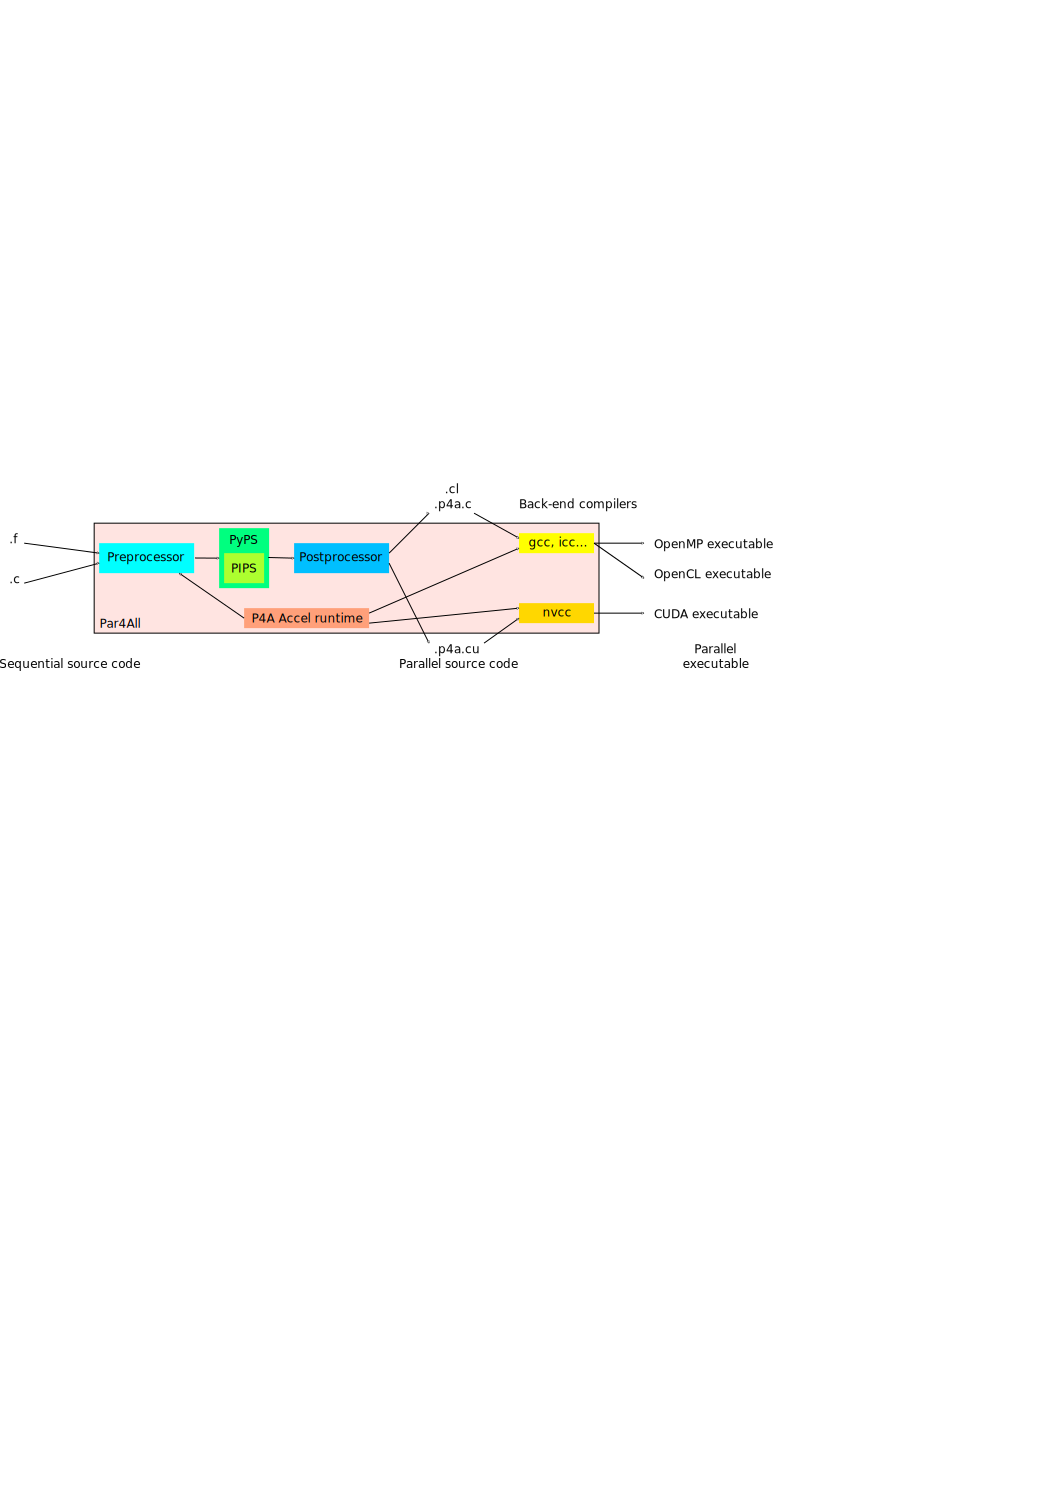
\includegraphics[width=\hsize]{p4a_work_flow.pdf}
  \caption{Intestinal view of \texttt{p4a}.}
  \label{fig:transit_intestinal}
\end{figure}

From the high-level user point of view, the sources follow this journey:
\begin{itemize}
\item the source files pass through the preprocessor of
  \Apips. C source files also pass through
  \verb|p4a_recover_includes| to instrument the
  \verb|#include| processing for later recovering;
\item the preprocessed files pass through a splitter that creates
  one file per function and a compilation unit file that keeps track
  of all the file-global declarations;
\item each function file or compilation-unit file can be parsed on
  demand according to the \Apyps script;
\item a predefined \Apyps program applies many different \Apips phases on
  the code and regenerate the transformed sources;
\item \verb|p4a_recover_includes| is applied again as a post-processor
  to recover most of the \verb|#include| work;
\item the sources are postprocessed by
  \verb|p4a_post_processor.py| to cope with some of the special syntax
  (\Acuda, \Aopencl...) that can not be directly represented in \Apips;
\item the generated final files are copied to the final directory;
\item if requested, the final target back-end compilers are called to
  produce the parallelized executable program.
\end{itemize}



\section{Examples and demos}
\label{sec:examples-demos}

The \texttt{examples} directory contains examples and benchmarks to
demonstrate the different features of \Apfa. Look at the local
\texttt{README.txt} for more information.

There are many more examples in the validation directory of \Apfa
(\S~\ref{sec:validation}), but they are less useful for training purposes.


\section{Validation}
\label{sec:validation}

The validation of \Apfa is done at different levels.

\subsection{Using PIPS validation}
Since \Apfa relies heavily on \Apips, the \Apips validation can be run
into the \texttt{package/PIPS/validation} directory of the \Agit working
copy. Refer to the validation section of the \Apips developer guide for
more information.

Note that since the validation relies on the presence of some directories,
old directories that may have been automatically created in the past but
are useless now may create parasitic failure entries in validation
results. So it may be useful to do a \texttt{git clean -d} in
\texttt{package/PIPS/validation} before running the \Apips validation.  It
is typically necessary also when validation directories have been moved
around in the \Apips \Asvn and this is not well managed at the \Agit level
since \Agit ignores empty directories.

There is a private validation in the \texttt{validation} directory of the
\texttt{par4all-priv} private directory. Refer to the
\texttt{par4all-priv/validation/README.txt} file to have documentation on
it. It is not explained in this document for confidentiality reasons.

It is mandatory for \Apfa developer to run the validation before pushing
big modifications to the reference \Agit server.

Since \Apips is a keystone in \Apfa, \Apips developers should verify that
their changes do not impact badly \Apfa by running the validation too, if
possible.\footnote{Even if many \Apips contributors are also \Apfa
  contributors, there are \Apips contributors not familiar nor even
  related with \Apfa.}


\subsubsection{\protect\texttt{p4a\_validate} utility}
\label{sec:p4a_validate-utility}


To facilitate validation, the \verb|p4a_validate|
script adds the concept of validation classes to the \Apips
validation. A class is a set of validation cases with common characteristics.

TODO: For example, there could be a class for \texttt{ALL} the
validation, for cases with the same result (e.g.,
\texttt{CHANGED}, \texttt{FAILED}, \texttt{PASS}, \verb|PREVIOUS_ALL|,
\verb|PREVIOUS_CHANGED|, \verb|PREVIOUS_FAILED|, \verb|PREVIOUS_PASS|),
etc. Once the classes are defined, set operations can be performed to combine
them (e.g., unions, intersections, etc.)

TODO: Other classes can be defined directly in the validation
directories with \texttt{.vclass} line-oriented regexp filter lines or with
generic Python code \texttt{.vclasspy}.

\verb|p4a_validate| has a small script interface, but the advanced
user desiring more interactivity
should use the Python classes directly, for example from \texttt{iPython}.

The first use of validation classes in \Apfa is to select from \Apips
only the test cases that pass the \Apips validation. This class can used to
construct a
\Amat (Minimal Acceptance Test) for \Apfa. Other \Apips validation
cases are more useful for \Apips developers, and are of less relevance
to \Apfa validation.

\subsubsubsection{Example}
\label{sec:example}

Use for example with 4 processes
\begin{verbatim}
make validate-out -j4
\end{verbatim}
that you can run:
\begin{itemize}
\item in one of the \texttt{validation} directory (from \Apips or in
  \texttt{par4all-priv}) to run all the validations cases defined in the
  \texttt{default} file and it generates a \texttt{SUMMARY.short} and
  archive it in the \verb|SUMMARY_Archive| directory;
\item in a sub-directory of the previous \texttt{validation} directory and
  it generates a \texttt{RESULTS} file in it.
\end{itemize}
In any case, \verb|p4a_validate| is to be used from a \texttt{validation}
directory and not from a subdirectory.

For more details on the validation process, look at the \Apips development
guide since we use its validation infrastructure.

To display from the last validation run only the test cases marked as
\texttt{changed} in \verb|C_syntax|, use:
\begin{verbatim}
p4a_validate --file=SUMMARY_Archive/SUMMARY-last --filter='^C_syntax/' \
             --keep-status=changed --list
\end{verbatim}

To show the test cases that changed in comparison to the reference output:
\begin{verbatim}
p4a_validate --file=SUMMARY_Archive/SUMMARY-last --filter='^C_syntax/decl' \
             --keep-status=changed --show-diff-files
\end{verbatim}

To accept the changed validation output in \texttt{C\_syntax/decl\emph{*}}
after a validation done from inside the \verb|C_syntax| directory:
\begin{verbatim}
p4a_validate --file=C_syntax/RESULTS --filter='^C_syntax/decl' \
             --keep-status=changed --accept
\end{verbatim}
When validation is complete, commit or revert to the previous state with \Agit.

If you have run validation
Occasionally, it is desirable to move all of the failed validation tests for
\texttt{Control} into a new validation directory \texttt{Control-Bugs} to
clean up the mainstream validation. This is accomplished with:
\begin{verbatim}
mkdir Control-Bugs
p4a_validate --file=RESULTS/SUMMARY  --list --filter=^Control/ --keep-status=failed \
 | sed -n -e 's,failed: ,,p' > files-to-move
\end{verbatim}
Once the state \texttt{files-to-move} is complete, the database is
cleaned with:
\begin{verbatim}
rm -rf Control/*.database
\end{verbatim}
and the test cases are moved with:
\begin{verbatim}
for f in `cat files-to-move` ; do git mv $f* Control-Bugs ; done
\end{verbatim}


\subsubsubsection{Option list of \protect\texttt{p4a\_validate}}
\label{sec:opti-list-p4a_v-1}

Below is a description of the usage and options for
\verb|p4a_validate|. The options are processed in the order of class
construction, filtering, display and acceptance, so that
actions can be piped. To track the differences between
multiple validations, \verb|pips_validate| should be run with the
\texttt{-k} (history keeping) option.

\input{p4a_validate-help}


\subsubsection{\texttt{p4a\_validate\_class.py} validation script}
\label{sec:validation_script}

The \verb|p4a_validate_class.py| python script is a front-end to \Apfa
validation and has several options for selecting validation tests.

Currently, available options are:
\begin{description}
\item[\texttt{--pips}:] validate tests which are done by default in
  \texttt{packages/PIPS/validation}

\item[\texttt{--p4a}:] validate tests which are done by
  \verb|par4all_validation.txt| (which exist in
  \texttt{src/validation})

\item[\texttt{--diff}:] compare the tests done with
  \texttt{--pips} and \texttt{--p4a} options. The list of the tests which
  are not done by \texttt{--p4a} options are included in \texttt{diff.txt}

\item[\texttt{--dir}:] Validate tests which are done in \verb|packages/PIPS/validation/directory_name|. Syntax is \verb|./p4a_validate_class.py --dir dir1 dir2 dir3|

\item[\texttt{--test}:] Validate tests which are given by the argument. Syntax is \verb|./p4a_validate_class.py --test directory_test/test.f| for example

\item[\texttt{-h} or \texttt{--help}:] Help for \verb|p4a_validate_class.py|
\end{description}

Examples with \verb|p4a_validate_class.py|:
\begin{verbatim}
python p4a_validate_class.py --pips
\end{verbatim}
or
\begin{verbatim}
python p4a_validate_class.py --p4a
\end{verbatim}

To use the option \texttt{--p4a}, a \verb|par4all_validation.txt| must be
previously created. This file lists all tests that the validation will do.
Syntax to add a new test is: \verb|directory_test/name_test|.

Be careful when adding a test to \verb|par4all_validation.txt|, put the
correct extension (\texttt{.c}, \texttt{.f}, \texttt{.F},
\texttt{.F90}). Don't use \texttt{.tpips}, \texttt{.tpips2}... extensions.

Example of a \verb|par4all_validation.txt| with 2 tests:
\begin{verbatim}
Syntax/alias.f
Syntax/altret01.f
\end{verbatim}

\subsection{Validation Par4All}

\section{Branches}
\label{sec:branches}

Since there are restrictions on the use of \texttt{/} in branch names,
it is preferable to use \texttt{-} to add hierarchy.

To facilitate development and organization, there are some already
defined branches:
\begin{description}
\item[\texttt{gcc-4.4.1}] is the original \Agcc 4.4.1 core \& Fortran in
  \texttt{package/pips-gfc};
\item[\texttt{gcc-4.4.2}] is the original \Agcc 4.4.2 core \& Fortran in
  \texttt{package/pips-gfc};
\item[\texttt{initial}] is the initial commit of the \Apfa
  repository. This branch is used
  to set the branches for the different packages and should not
  be used for development.
\item[\texttt{p4a-\emph{numerical}}] is a branch corresponding to a
  given version snapshot;
\item[\texttt{p4a-\emph{numerical}-alpha}] is a branch corresponding
  to an alpha version of a given version snapshot;
\item[\texttt{p4a-\emph{numerical}-beta}] is a branch corresponding to a beta
  version of a given version snapshot;
\item[\texttt{p4a}] is the branch to get the full latest \Apfa version
  with all the different components, which is the merge of the branches
  \texttt{p4a-own} and \texttt{p4a-packages};
\item[\texttt{p4a-linear}] points to the import of \Apips \texttt{linear}
  part. Therefore, this branch should contain only files from
  \texttt{package/PIPS/linear} and is the merge source for
  the last version from \texttt{linear};
\item[\texttt{p4a-newgen}] points to the import of the \Apips \texttt{newgen}
  part and should contain only files from
  \texttt{package/PIPS/newgen};
\item[\texttt{p4a-nlpmake}] points to the import of \Apips \texttt{nlpmake}
  part and should contain only files from
  \texttt{package/PIPS/nlpmake};
\item[\texttt{p4a-own}] points to the last development of the \Apfa files,
  without packages, etc;
\item[\texttt{p4a-packages}] points to the last merge of all the \Apfa
  package components;
\item[\texttt{p4a-pips}] points to the import of the \Apips \texttt{pips}
  part. Therefore, this branch should contain only files from
  \texttt{package/PIPS/pips} and is the merge source for
  the last version from \texttt{pips};
\item[\texttt{p4a-polylib}] points to the import of the \Apips \texttt{polylib}
  part. Therefore, this branch should contain only files from
  \texttt{package/polylib} and is the merge source for
  the last version from \texttt{polylib};
\item[\texttt{p4a-validation}] points to the import of the \Apips
  \texttt{validation} part and consists only of file from
  \texttt{package/PIPS/validation};
\item[\texttt{pips-gfc+gcc}] points to a working \Apipsgfc implementation
  of the Fortran 95 extension for \Apips in \texttt{package/pips-gfc};
\item[\texttt{pips-gfc-4.4.1}] points to the original developments of
  Raphaël in \Agcc in \texttt{package/pips-gfc}.
\end{description}

For tractability, there are also branches that point
to specific versions of particular branches such as
\texttt{p4a-0.2-alpha-nlpmake}, \texttt{p4a-own-0.1} or
\texttt{p4a-packages-0.2-beta}.


\section{Useful \protect\Agit tricks for \protect\Apfa}
\label{sec:some-agit-tricks}

\subsection{Files committed to the wrong branch}
\label{sec:you-have-comited}

There are (too) many branches in \Apfa, right? Distinguishing the many
branches of \Apfa is complicated; for example, it is easy
to commit to the \texttt{p4a} branch instead of the correct
\texttt{p4a-own} branch. The good news is that since \Agit separates
the commit and publish phases, one can examine the history
with tools such as \texttt{gitk} to find errors before negatively
impacting your colleagues.

Here is an example of a wrong \texttt{p4a} commit and how to achieve a
good state before pushing to the public repository.

First create a branch to facilitate tracking:
\begin{verbatim}
git checkout -b wrong
\end{verbatim}
Return to a clean state (use only 1 \verb|^| to return to the previous
commit):
\begin{verbatim}
git branch -f p4a p4a^
\end{verbatim}
Move the incorrect commit to the correct branch:
\begin{verbatim}
git rebase --onto p4a-own p4a wrong
\end{verbatim}
Then go to the target branch:
\begin{verbatim}
git checkout p4a-own
\end{verbatim}
and merge the current work into it:
\begin{verbatim}
git merge wrong
\end{verbatim}
and delete the helping branch:
\begin{verbatim}
git branch -d wrong
\end{verbatim}
Magic isn't it? \smiley

The wrong work is still connected to the branch
\texttt{p4a}, but no longer \emph{in} the branch. It is typical in
\Agit to avoid the loss
of information.


\subsection{The history has been rewritten on the server or how to resolve
  an uchrony with git}
\label{sec:history-has-been}

\Apfa is complex with many branches and sometimes some commits that should
have not existed reach the development server. For example, when an error
should have been fixed as in section~\ref{sec:you-have-comited}
\emph{before} pushing on the server...

In this case, someone change the head of the wrong branches on the server
and a mail is sent to the developer list to warn everybody that the
branches have been sent back in the past to discard some commits. In
general the action to do, if you have not committed new stuff since this
event on this branch, is something like:
\begin{verbatim}
git fetch
git branch -f p4a <some nice SHA-1 value>
\end{verbatim}

In the general case, if you have not done some developments since the
history rewriting of the \texttt{p4a} branch for example, you can try:
\begin{verbatim}
git fetch
git branch -f p4a remotes/origin/p4a
\end{verbatim}
to make the local tracking branch to the server branch.

If you want to resynchronize all the branches, try:
\begin{verbatim}
# First park to a third-party unused branch to avoid interferences:
git checkout master
git fetch
p4a_git --branch-action git branch -f p4a\$suffix remotes/origin/p4a\$suffix
\end{verbatim}

The following is for people willing to understand what can happen.

If you do not do that what is going to happen? If no new commit is pushed
on the server and you push candidly tour repository, the previously
fetched wrong commits will be sent back to the server since you are in the
future compared to the new reference on the server (which we sent back in
the past by rewriting the history, do you remember?). Since \Agit is a
peer-to-peer system, your repository or the central repository are
considered of the same importance and yours is trusted as so. So the wrong
commits will appear back in the central repository where they will
reappear for everybody... \frownie{} Then, everybody recurse at the
beginning of section~\ref{sec:history-has-been}... Too bad.

If there has been some new commits on the server, the server branch is in
some future compared to the point the server branch was sent back in the
past but your branch (which is in the previous future \smiley) seems
having diverged since this point. So if you do a \texttt{git pull}, the
automatic merge is likely to fail. This is why you have to reset manually
the reference branch with a \texttt{git branch -f} as previously
explained.

In the worst case, you have committed some work before figuring out the
history has been rewritten. Then you can create a new branch to point on
your work. Then you can sent back the wrong branch in the past. Then you
pull from the server and you can apply back your commits by cherry-picking
from the save branch or rebasing it as in
section~\ref{sec:you-have-comited}.

Have you still done something quite wrong? It is not an issue, everything
is done in \Agit to avoid losing work. It is somewhere. Just figure out
where and how to get back on rails. \smiley

\begin{quote}
  To summarize this section, you need to understand that rewriting the
  history is globally a pain for everybody in the project. So, since a
  nice feature of \Agit is to separate commits from pushing to a server,
  take some times to review commits \emph{before} pushing them. If this is
  not respected, we will forbid direct commits to the central server but
  we will use quarantine server or branches first.
\end{quote}


\appendix

\section{Various script details}
\label{sec:vari-script-deta}

In this appendix, options and other ancillary scripts are described.

\subsection{The \protect\texttt{p4a\_recover\_includes} script}
\label{sec:p4a_recover_includes}

\verb|p4a_recover_includes| is used to get C standard \verb|#include|
after \Apips digestion to have a smoother recompilation (for \Acuda it is a
requirement) and more readable code without ugly macro inclusions at
the beginning of all the files.

This script can also be used to do expansion of the \verb|#include| of
\Apfa Accel to see the \Acuda or \Aopenmp code
that is generated.

\input{p4a_recover_includes-help}


\subsection{The \protect\texttt{p4a\_post\_processor.py} script from
  Par4All Accel}
\label{sec:p4a_p-script-from}

\verb|p4a_post_processor.py| transforms the \Apips
output into calls to \Apfa Accel. It is mainly used by the \texttt{p4a}
script but can be used by advanced users who need to write their own
specialized \Apips scripts with \texttt{tpips} or \texttt{PyPS}.

\input{p4a_post_processor.py-help}


\subsection{The \protect\texttt{optparse\_help\_to\_tex} help
  documentation to \TeX{} compiler}
\label{sec:help-docum-tex}

\verb|optparse_help_to_tex| is a small compiler that translates a help
output message of a command launched with \texttt{-h} using the
\texttt{optparse} format when into La\TeX{} code with section for
inclusion in
an article or slide generation with Beamer.

The following section should be a very demonstration of this tool
indeed. \smiley

\input{optparse_help_to_tex-help}

\section{Tools, tips and tricks for developpers}

%%ContentEnd

\end{document}


%%% Local Variables:
%%% mode: latex
%%% ispell-local-dictionary: "american"
%%% End:
